\subsection{离散时间傅里叶变换}

\subsubsection{数字信号与数字频谱}


\begin{exercise}
    已知 $f(t)$ 的频谱函数为 $F(\omega)$,试证明:
    \begin{align*}
        T \cdot \sum_{n = -\infty}^{+\infty}f(nT_s) = \sum_{k = -\infty}^{+\infty}F(k\omega_s),
    \end{align*}
    其中 $\omega_s = 2\pi / T_s$。
\end{exercise}

\begin{proof}
    由于
    \begin{align*}
        \hat{F}(\omega) = \frac{1}{T_s}\sum_{m = -\infty}^{+\infty}F(\omega - m\omega_s),
    \end{align*}
    且
    \begin{align*}
        \hat{F}(\omega) = \sum_{n = -\infty}^{+\infty}f(nT_s)\mathe^{-\mathi\omega nT_s},
    \end{align*}
    故当 $\omega = 0$ 时,有
    \begin{align*}
        \frac{1}{T_s}\sum_{m = -\infty}^{+\infty}F(-m\omega_s) & = \hat{F}(0) \\
        & = \sum_{n = -\infty}^{+\infty}f(nT_s) \cdot \mathe^{0} \\
        & = \sum_{n = -\infty}^{+\infty}f(nT_s).
    \end{align*}
    此即
    \begin{align*}
        T_s \cdot \sum_{n = -\infty}^{+\infty}f(nT_s) = \sum_{m = -\infty}^{+\infty}F(-m\omega_s).
    \end{align*}
    命题得证。
\end{proof}

\subsubsection{离散时间傅里叶变换的性质}



\subsubsection{有限长离散时间傅里叶变换}

假设有信号 $x(n)$,其离散时间傅里叶变换为 $X(\omega)$。
由于计算机只能存储有限长的信息,因此我们考虑使用长度为 $L$ 的窗函数
\begin{align*}
    w(n) = \begin{cases}
        1, & 0 \le n \le L-1, \\
        0, & n \ge L \text{ 或 } n < 0
    \end{cases}
\end{align*}
将信号限制在有限长区间内,得到 $x_L(n)$,即
\begin{align*}
    x_L(n) = x(n)w(n) = \begin{cases}
        x(n), & 0 \le n \le L-1, \\
        0, & n \ge L \text{ 或 } n < 0.
    \end{cases}
\end{align*}
接下来,我们将讨论经过窗函数处理后的信号的
离散时间傅里叶变换 $X_L(\omega)$。

\begin{example}
    第一种方法是直接带入 DTFT 公式进行求解。由定义知
    \begin{align*}
        X(\omega) = \sum_{n = -\infty}^{+\infty}x(n)\mathe^{-\mathi\omega n}.
    \end{align*}
    因此,有
    \begin{align*}
        X_L(\omega) & = \sum_{n = -\infty}^{+\infty}x_L(n)\mathe^{-\mathi\omega n} \\
        & = \sum_{n = 0}^{L-1}x(n)\mathe^{-\mathi\omega n}.
    \end{align*}
    注意此时求和的上限是 $L-1$,而不是 $+\infty$。
\end{example}

\begin{example}
    第二种方法是利用卷积定理。由卷积定理,我们知道
    求数字域上的乘积等价于在频域上进行圆卷积。因此
    \begin{align*}
        X_L(\omega) & = \frac{1}{2\pi}X(\omega) \otimes W(\omega) \\
        & = \frac{1}{2\pi}\int_{-\pi}^{\pi}X(\omega')W(\omega - \omega')\D{\omega'}.
    \end{align*}
\end{example}

\begin{example}[窗函数的频谱与主瓣宽度]
    窗函数 $w(n)$ 的 DTFT 为
    \begin{align*}
        W(\omega) & = \sum_{n = -\infty}^{+\infty}w(n) \mathe^{-\mathi\omega n} \\
        & = \sum_{n = 0}^{L-1}\mathe^{-\mathi\omega n} \\
        & = \frac{1 - \mathe^{-\mathi\omega L}}{1 - \mathe^{-\mathi\omega}} \\
        & = \frac{\sin(\omega L/2)}{\sin(\omega/2)}\mathe^{-\mathi\omega(L-1)/2}.
    \end{align*}
    因此,画出它的频谱如 \ref{fig:DTFT_window.png} 所示。
    \begin{figure}[H]
        \centering
        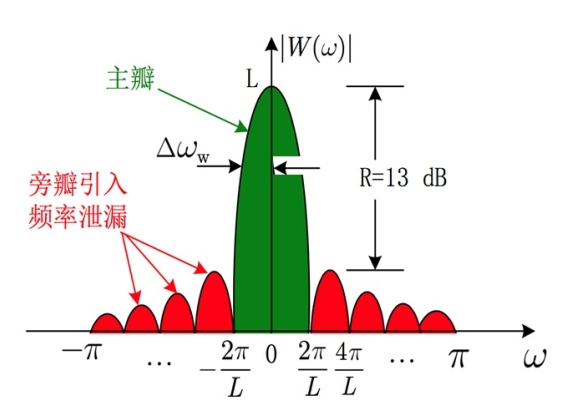
\includegraphics[width=0.6\textwidth]{chap3/img/DTFT_window.png}
        \caption{窗函数的频谱}
        \label{fig:DTFT_window.png}
    \end{figure}
    为方便起见,我们定义它的\bd{主瓣宽度}为
    \begin{align*}
        \Delta\omega_W = \frac{2\pi}{L}.
    \end{align*}
\end{example}

\subsubsection{频谱分辨率}

\begin{example}
    给定信号
    \begin{align*}
        x(n) = A_1\mathe^{\mathi\omega_1 n} + A_2\mathe^{\mathi\omega_2 n},
    \end{align*}
    其中 $n \in \set{Z}, 0 < \omega_1 < \omega_2 < \pi$,
    在一个奈奎斯特区间内,它的 DTFT 为
    \begin{align*}
        X(\omega) = 2\pi(A_1\delta(\omega - \omega_1) + A_2\delta(\omega - \omega_2)).
    \end{align*}
    画出它的频谱如 \ref{fig:DTFT_two_freqs.png} 所示。
    \begin{figure}[H]
        \centering
        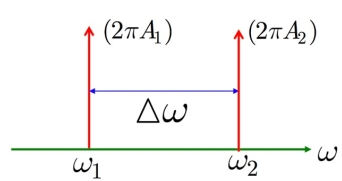
\includegraphics[width=0.3\textwidth]{chap3/img/DTFT_two_freqs.png}
        \caption{两个频率的信号的频谱}
        \label{fig:DTFT_two_freqs.png}
    \end{figure}
    可以看出,这两个频率的间隔为 $\Delta\omega = \omega_2 - \omega_1$。
\end{example}

\begin{example}
    给定信号
    \begin{align*}
        x_L(n) = A_1\mathe^{\mathi\omega_1 n} + A_2\mathe^{\mathi\omega_2 n},
    \end{align*}
    其中 $n \in [0, L-1], 0 < \omega_1 < \omega_2 < \pi$,
    在一个奈奎斯特区间内,它的 DTFT 为
    \begin{align*}
        X_L(\omega) & = \frac{1}{2\pi}X(\omega) \otimes W(\omega) \\
        & = A_1W(\omega - \omega_1) + A_2W(\omega - \omega_2).
    \end{align*}
    画出它的频谱如 \ref{fig:DTFT_two_freqs_window.png} 所示。
    \begin{figure}[H]
        \centering
        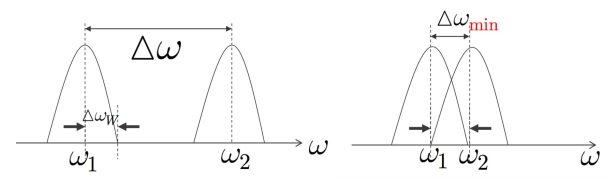
\includegraphics[width=0.6\textwidth]{chap3/img/DTFT_two_freqs_window.png}
        \caption{两个频率的信号的频谱}
        \label{fig:DTFT_two_freqs_window.png}
    \end{figure}
    可以看出,这两个频率的间隔为 $\Delta\omega = \omega_2 - \omega_1$。
\end{example}

\begin{definition}[频谱分辨率]
    那么当 $\Delta\omega$ 很小时,我们如何判断两个频率之间的距离呢?
    或者换而言之,要求分辨出这两个频率,$\Delta\omega$ 至少要多大呢?
    这就引出了\bd{频谱分辨率}的概念。

    当 $\Delta\omega$ 不小于窗函数的主瓣宽度 $\Delta\omega_W = 2\pi/L$ 时,
    我们认为可以分辨出两个频率。也就是说,定义 DTFT 的\bd{频谱分辨率}为
    \begin{align*}
        \Delta\omega_{\min} = \Delta\omega_W = \frac{2\pi}{L},
    \end{align*}
    其中 $L$ 是窗函数的宽度(即序列的长度)。
\end{definition}

\begin{remark}
    序列加窗后会对频谱产生两种影响:
    \begin{enumerate}
        \item 序列频谱中可分辨的最小频率间隔由数据长度决定,
            即窗函数的时间长度。这个现象被称为\bd{不确定原理}。
        \item 序列频谱中出现了高频分量。它们是由于矩形窗
            两个边缘处的突变所造成的。这个现象被称为\bd{频率泄漏}。
            好像是这些原来谱中没有的高频成分是从``内部''(信号原谱分布区间)中
            ``泄漏''出来的一样。显然,这些泄漏量与窗函数的旁瓣有关系,如
            图 \ref{fig:DTFT_leakage.png} 所示。
            \begin{figure}[H]
                \centering
                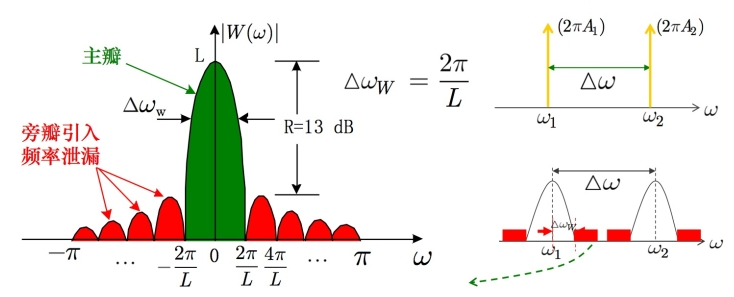
\includegraphics[width=0.6\textwidth]{chap3/img/DTFT_leakage.png}
                \caption{频率泄漏}
                \label{fig:DTFT_leakage.png}
            \end{figure}
    \end{enumerate}
\end{remark}
